% !TeX root = Bericht.tex
% !TeX spellcheck = en_US
\section{Results}
In this section, all results of the experiments are presented, including all relevant analysis. 
\subsection{Measurement of the electronic
	components and the optimum Bragg
	angle}\label{bragg_angle_berechnung}

Due to geometric considerations, the Bragg angle $\theta_{\mathrm{B}}$ was calculated as $\theta_{\mathrm{B}} = \arctan(d_{01}/2d)$, where $d_{01} = 0.8(1) \unit{cm}$ is the length difference between \nth{0} and \nth{1} order diffracted beams at the powermeter, and $d = 61.2(3) \unit{cm}$ is the total path length from the AOM to the powermeter. This results in
$$\theta_{\mathrm{B}} = 6.5(8) \unit{mrad}.$$ 
The high uncertainty is a direct consequence of the big uncertainty in the measurement of the length difference between zeroth and first diffraction order, which was hard to measure exactly. \newline

In order to determine a exact conversion from the peak-to-peak Voltage in mVpp, which is set at the powermeter, to the RF-power in $\oldunit{mW}$, we use a table given in \autocite{UmrechnungsTabelleDB}. We plotted power for the given voltage in the first column of the table, and fitted a quadratic function, as seen in \autoref{fig:umrechnung_plot}. This function type had the best fit quality  with a $\chi_\nu$ well below 1, which when dealing with uncertain measurements indicates that the theory fits the data \blockquote{too well} (here we have no uncertainty so a small $\chi_\nu$ is expected).
\begin{figure}[H]
	\centering
	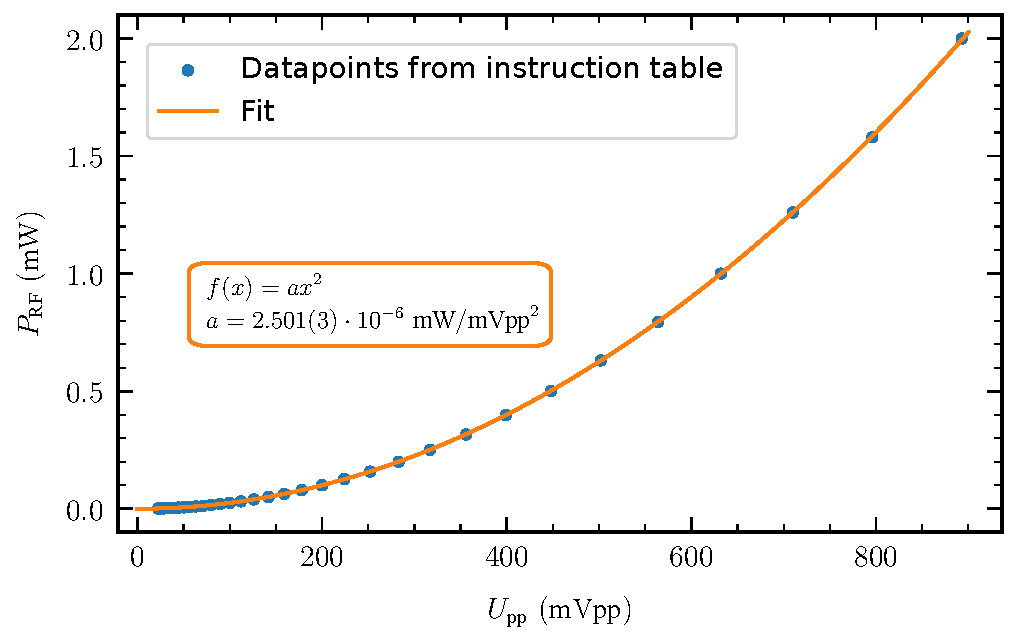
\includegraphics[width=\textwidth]{umrechnung}
	\caption{The data points plotted are the given values out of the transformation table in \autocite{UmrechnungsTabelleDB}. A quadratic function with given fit parameters helps us transforming values from peak-to-peak-voltage to RF-power. }
	\label{fig:umrechnung_plot}
\end{figure}

\subsection{Measurement of the intensity dependence and determination of the saturation power}
Without applied RF-power, the insertion loss $IL$ was determined using the formula given in \autoref{subsec:AOM}. With $\P{in}= 0.877(5) \unit{mW}$ and $\P{out} = 0.791(5) \unit{mW}$ we get
$$IL = 0.098(8).$$

In \autoref{fig:plot_saturation_power}, measured efficiency $\varepsilon = \P{i}/\P{out}$, with i representing different diffraction orders, is plotted in dependence of the RF-power. A fit based on \autoref{eqn:epsilon2} is done for the first diffraction order. 
\begin{figure}[H]
	\centering
	\begin{tikzpicture}
		\begin{scope}[xshift=1.5cm]
			\node[anchor=south west,inner sep=0] (image) at (0,0) {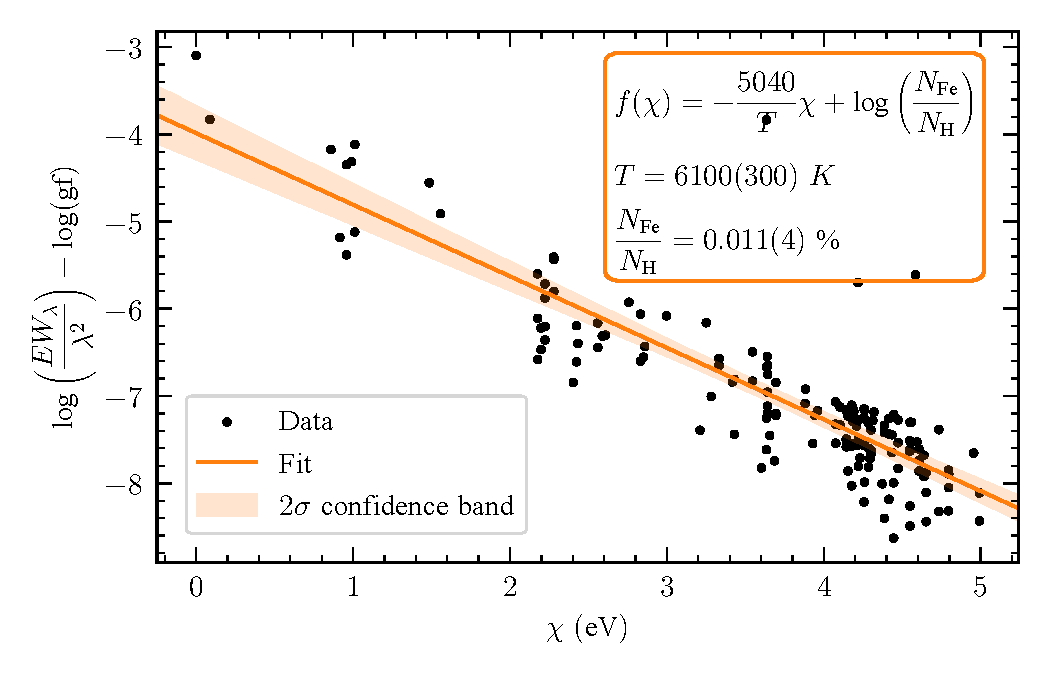
\includegraphics[width=\textwidth]{fit}};
			\begin{scope}[x={(image.south east)},y={(image.north west)}]
				\node[draw=MyBlue, rounded corners, ultra thick, align=left] at (0.65, 0.62) {$f(x) = a \cdot \sin^2\left(\frac{\pi}{2} \sqrt{x/\P{sat}}\right)$\\
					$a = 0.915(16)$\\
					$\P{sat} = 1.21(3) \unit{\watt}$};
			\end{scope}
		\end{scope}
	\end{tikzpicture}
	\caption{The measured efficiency of the \nth{0} and \nth{1} diffraction orders is shown with varying RF power. On the top x-Axis the values set in the frequency generator are shown, whilst the bottom x-Axis shows the converted power after the amplifier. The errors of the efficiencies are just too small to make out (they are of the order of the dot size). \nth{1} order data was used to fit a $\sin^2$ law, which is shown as blue line with $2\sigma$ confidence band.} 
	\label{fig:plot_saturation_power}
\end{figure}

From this fit, we can extract the saturation power and we get 
$$\P{sat} = 1.21(3) \unit{W}.$$


\subsection{Measurement of the frequency
	dependence and determination of the
	quality factor}\label{frequency_dependence}
In \autoref{fig:plot_qualityfactor1}, the measured efficiency is plotted for varying frequency \frf from \SI{60}{MHz} to \SI{100}{MHz}. The uncertainty in frequency is neglected, as we assume it to be much smaller than the uncertainty of the measured power. Thus, its influence can be ignored. In \autoref{fig:plot_qualityfactor1} the measured efficiency of the \nth{1} diffraction order is plotted against frequency. From \autoref{eqn:epsilon} we expect the efficiency to follow a $\sin(x)/x$ relation with regards to frequency. This function has been fitted to the data and can also be seen in \autoref{fig:plot_qualityfactor1}. The parameters were expressed in a way such as to give them a physical meaning. 
\begin{figure}[H]
	\centering
	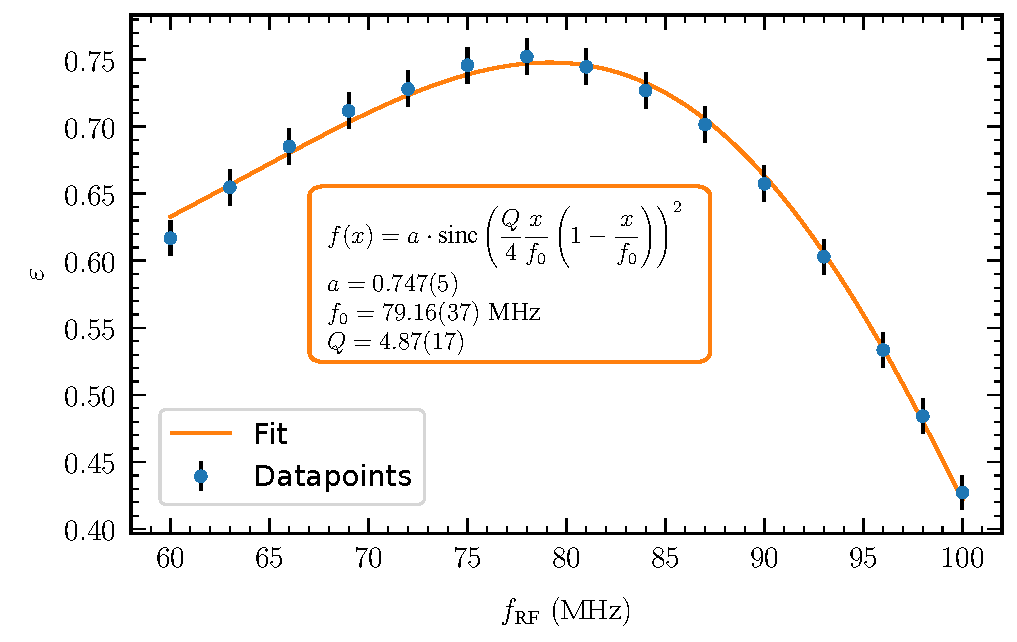
\includegraphics[width=\textwidth]{sincfit}
	\caption{The measured efficiency dependent on frequency is shown. In addition, a fit is given, from which we can deduce a fitted central frequency $f_0$ and the quality factor $Q$.} 
	\label{fig:plot_qualityfactor1}
\end{figure}
Even though the resonant frequency of the AOM is listed in \autocite{bragg} to be \SI{80}{MHz}, we chose to include it as a free parameter in the fit, since AOMs can drift in frequency. It turns out our AOM with $f_0 = 79.16(37)\unit{MHz}$ is within $2 \sigma$ of the manufacturers value so in the future, fitting can be done without leaving this parameter free. Additionally we get a quality factor of
$$Q_1=4.87(17) .$$

Furthermore, the change of the Bragg angle depending on the RF frequency is investigated. In \autoref{fig:winkel_linear_plot}, Bragg angle $\theta_\mathrm{B}$ is plotted against frequency \frf. Again, the frequency is assumed to be perfect and only uncertainties from determining the angle matter.
\begin{figure}[H]
	\centering
	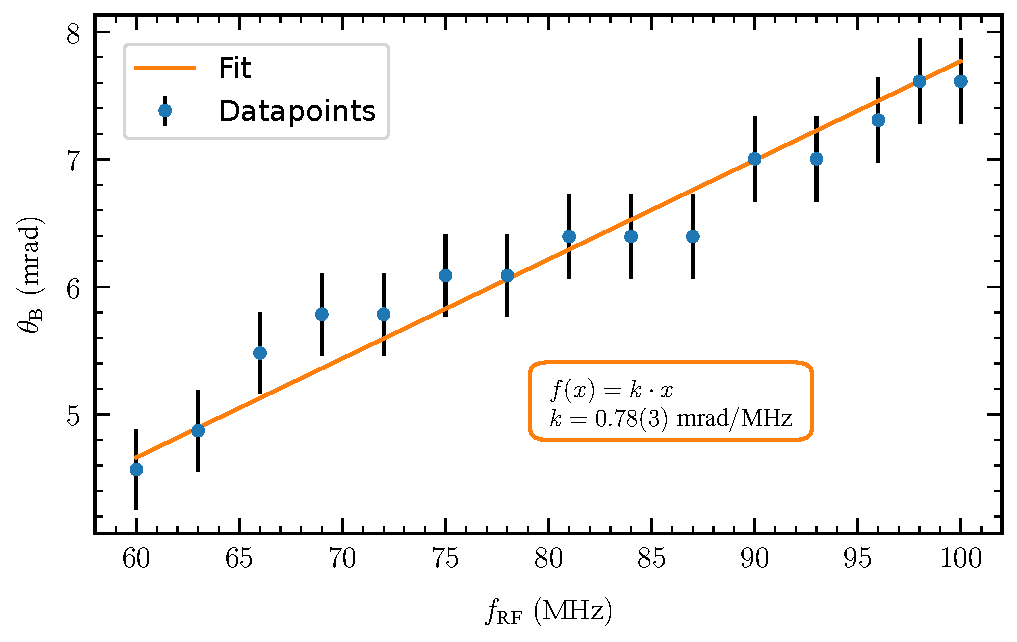
\includegraphics[width=\textwidth]{braggwinkel}
	\caption{On the x-axis of this plot, frequency is plotted, whereas on the y-axis, the matching Bragg angle is shown. Furthermore, a linear fit is done through the data points.} 
	\label{fig:winkel_linear_plot}
\end{figure}

As can be seen in the plot, the Bragg angle is increasing linearly with frequency. This is supported by a linear fit that describes the data points well. The discrete jumps in angle can be attributed to the millimeter ticks on the measuring tape, which were the smallest . 


\subsection{Measurement of the angle dependence and comparison of the quality factor}
Now a different technique is used to determine the quality factor. This time, the angle of the AOM is adjusted around its optimum value by $\pm\ang{1}$. We used the ticks on the micrometer screw of the rotating mount, which then have to be converted into angles. 
In figure \autoref{fig:plot_qualityfactor2}, the measured efficiency is plotted against the normalized angle difference $\Delta$, which is defined as the deviation from the optimal angle, divided by the Bragg angle calculated in \autoref{bragg_angle_berechnung}. \autoref{eqn:epsilon2} predicts again a $\sin(x)/x$ dependence, which was fitted and can also be seen in in \autoref{fig:plot_qualityfactor2}.
\begin{figure}[H]
	\centering
	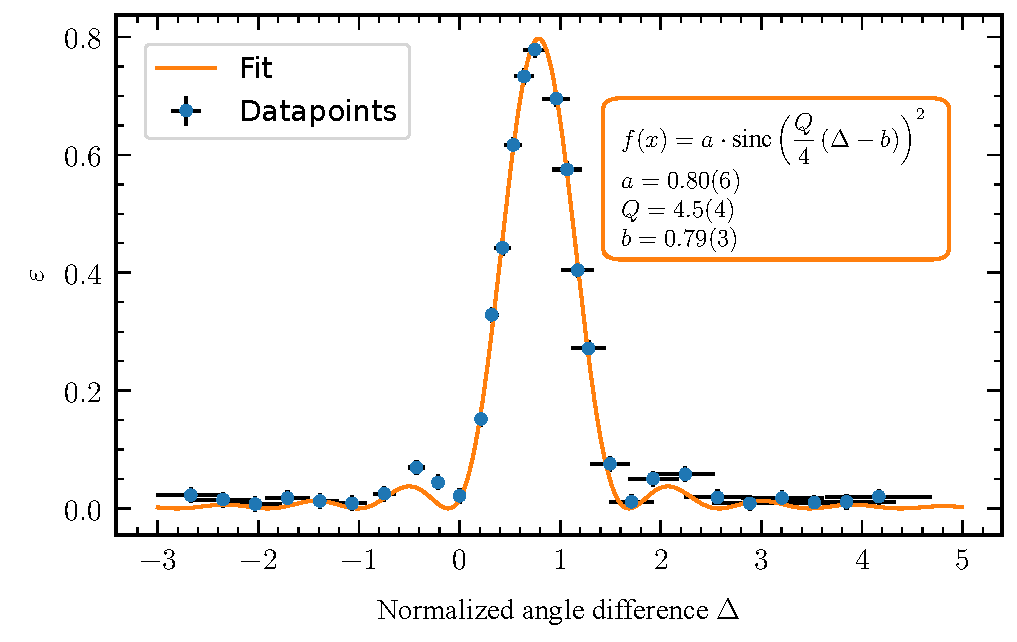
\includegraphics[width=\textwidth]{deltasinc}
	\caption{The efficiency is plotted depend in the normalized angle difference. A fit-function, described in the plot, is shown too. } 
	\label{fig:plot_qualityfactor2}
\end{figure}
We included the parameter $b$ in the fit to catch systematic shifts due to the rotation mounts deadzone. From visual inspection we estimated it to be 5 ticks, the fit returns a value of $b = 7.37(4) \unit{ticks}$.
Using the fit, we get a quality factor of
$$Q_2 =  4.5(4).$$


\subsection{Measurement of the angular dependence of the maximum diffraction efficiency}
In this part of the experiment, the RF frequency is varied from \SI{60}{MHz} to \SI{100}{MHz}, but in contrast to \autoref{frequency_dependence}, the Bragg angle is adjusted to maximise the efficiency. From these results we see how the maximum efficiency is behaving, depending on the RF frequency. In \autoref{fig:plot_winkel}, the maximum efficiency is plotted against the RF frequency. 
\begin{figure}[H]
	\centering
	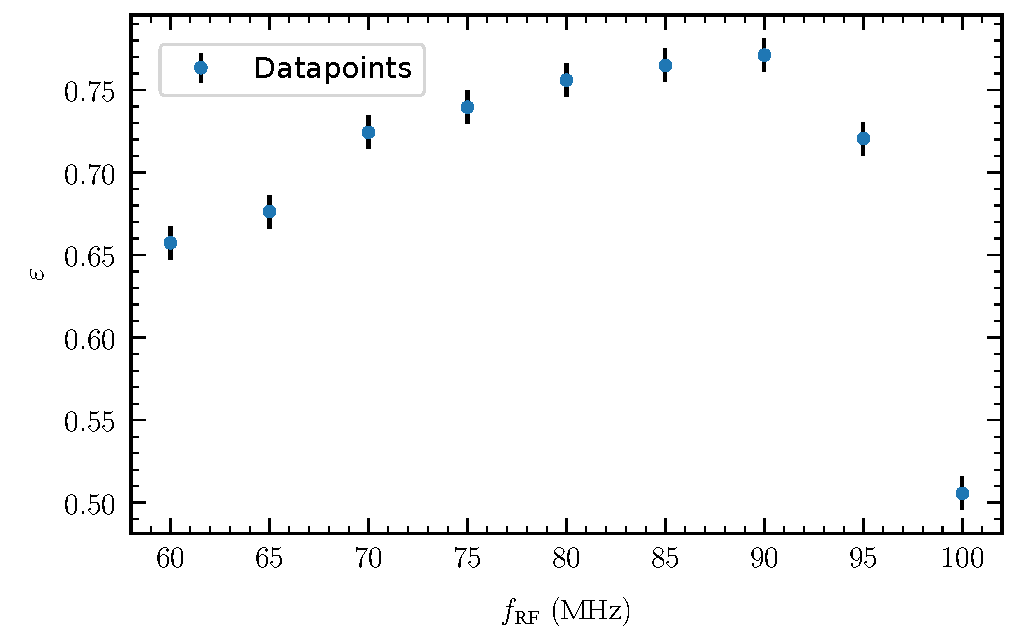
\includegraphics[width=\textwidth]{plot5}
	\caption{The maximum received efficiency, with optimised Bragg angle, is shown in dependence of the RF frequency \frf. } 
	\label{fig:plot_winkel}
\end{figure}